\documentclass[11pt]{article}
\usepackage[margin=1in]{geometry}
\usepackage{booktabs}
\usepackage{amsmath}
\usepackage{graphicx}
\usepackage{hyperref}
\usepackage{xcolor}
\usepackage{algorithm}
\usepackage{algpseudocode}
\usepackage{multirow}
\usepackage{caption}
\usepackage{tikz}
\usetikzlibrary{arrows.meta, positioning, shapes.geometric, fit, calc}

\title{PRISM: Policy-Ranked Reflective Memory for Safe LLM Agents}

\author{Sahil Soni}

\date{}

\begin{document}
\maketitle

% ============================================================================
\begin{abstract}
LLM agents deployed in production must respect domain policies.
We find that including policies in the system prompt produces high but
unverifiable compliance: models self-comply 80--90\% of the time, and
advisory approaches (RAG, Reflexion) reach 82--93\%, but no advisory
approach can verify that a specific rule was enforced on a specific action.
We present PRISM (Policy-Ranked Injection with Stratified Memory),
a memory architecture that separates policy discovery, failure-derived
rule promotion, and deterministic enforcement through three mechanisms:
(1)~policy memory with human-curated rules,
(2)~crystal memory where rejected actions are promoted into reusable
safety rules with evidence-based trust scores,
and (3)~a formal trust ordering where higher-trust memory overrides
lower-trust suggestions before tool execution, without LLM reasoning
in the loop.
We evaluate PRISM on PRISM-Bench (80 tasks, retail and airline domains)
with two resolver implementations: regex-based pattern matching and
FTS5 keyword matching.
PRISM-regex achieves $85.2\% \pm 1.0\%$ retail and $90.7\% \pm 2.5\%$
airline task success with zero over-blocking but limited recall.
PRISM-FTS5 improves violation recall but introduces 65\% over-blocking
on airline tasks due to proposal-refusal ambiguity.
The architecture contribution---trust-ordered tiers with failure-to-rule
promotion and deterministic conflict resolution---is independent of the
matcher. The gap between regex (too narrow) and FTS5 (too broad) defines
the open grounding problem for deterministic LLM policy enforcement.
All tasks, rules, prompts, raw outputs, and evaluation scripts are released.
\end{abstract}

% ============================================================================
\section{Introduction}
\label{sec:intro}

LLM agents are increasingly deployed in production customer-service, financial, and regulatory settings
where adherence to domain-specific policies is not optional~\cite{yao2023react,shinn2023reflexion}.
A retail agent must refuse to cancel shipped orders.
An airline agent must not rebook economy tickets within 24 hours of departure.
Violations carry real costs: regulatory fines, customer harm, and organizational liability.

The standard approach is to include policies in the system prompt
and rely on the model to self-enforce them.
Our experiments show this works surprisingly well---LLMs self-comply with prompt-level policy
79--96\% of the time depending on domain and context (Table~\ref{tab:comply}).
Retrieval-augmented generation (RAG) and Reflexion-style episodic
memory~\cite{shinn2023reflexion} improve this to 82--93\% task success.

However, high average compliance is insufficient for safety-critical deployment.
The problem is not that LLMs usually ignore policy---they usually follow it.
The problem is that \emph{which actions violate policy is unpredictable and unverifiable per-action}.
A system that follows policy 98\% of the time cannot tell you
which 2\% it will miss, cannot prove that a specific rule was enforced on a specific action,
and cannot provide an audit trail linking enforcement decisions to their justification.

We present PRISM (\textbf{P}olicy-\textbf{R}anked \textbf{I}njection with \textbf{S}tratified \textbf{M}emory),
a memory architecture that adds deterministic, auditable policy enforcement to LLM agents.
PRISM does not replace the LLM's reasoning---it adds a pre-action enforcement layer
that enforces every action matching an encoded rule before execution.
PRISM organizes agent memory into three tiers with a formal trust ordering:

\begin{enumerate}
\item \textbf{Policy Memory (T1):} Human-curated rules with deterministic pattern-based blocking.
      Trust = 1.0. Always loaded.
\item \textbf{Crystal Memory (T3):} Failure-derived rules promoted from rejected agent actions,
      with evidence-based trust scores. Trust = 0.5--0.95. Active after reaching
      an activation threshold ($\geq 0.70$).
\item \textbf{Episodic Memory (T2):} Retrieved past cases and domain knowledge.
      Trust = 0.70. Retrieved at query time.
\end{enumerate}

The trust ordering is deterministic: $\text{T1} > \text{T3} > \text{T2}$.
Higher-trust memory blocks lower-trust suggestions before tool execution.
The LLM reasons within these constraints but does not decide which memory wins.

Our contribution is not tiered memory---MemGPT~\cite{packer2023memgpt} and others already do that.
Our contribution is not failure-derived memory---Reflexion~\cite{shinn2023reflexion} already does that.
Our contribution is \emph{the combination of deterministic trust-ordered conflict resolution
with failure-to-rule promotion}, producing an enforcement system where:

\begin{itemize}
\item Every enforcement decision is deterministic and traceable to a specific rule.
\item Rejected actions are converted into structured blocking rules (Crystal memory),
      not advisory reflective text.
\item Crystal rules earn trust through evidence and can be audited, overridden, or promoted.
\end{itemize}

We evaluate PRISM on PRISM-Bench, an 80-task synthetic policy-compliance benchmark
inspired by $\tau$-bench-style~\cite{yao2024taubench} retail and airline workflows,
using a five-configuration ablation (C0--C4) that isolates each component's contribution.
We report honest results: RAG and Reflexion-style memory sometimes outperform PRISM on raw task success,
and no pairwise accuracy differences reach statistical significance at our sample sizes.
PRISM's value is not always higher accuracy---it is the change from
\emph{advisory compliance} to \emph{deterministic, auditable enforcement}.
All tasks, labels, rules, prompts, raw model outputs, and evaluation scripts are
released for full reproducibility.

% ============================================================================
\section{Related Work}
\label{sec:related}

\paragraph{Agent memory systems.}
MemGPT~\cite{packer2023memgpt} introduces virtual context management via memory paging,
enabling LLM agents to manage information beyond the context window.
Zep~\cite{zep2024} uses temporal knowledge graphs for agent memory.
A-MEM~\cite{amem2024} dynamically organizes memory networks.
MIRIX~\cite{mirix2024} optimizes memory-indexed retrieval.
These systems optimize \emph{what to remember} and \emph{when to retrieve}.
None provides trust-ordered conflict resolution or deterministic pre-action blocking.

\paragraph{Reflexion and failure-derived memory.}
Reflexion~\cite{shinn2023reflexion} demonstrated that agents can learn from task feedback
by storing reflective text summaries in episodic memory for future trials.
Hindsight~\cite{hindsight2024} provides retrospective memory for task improvement through post-hoc analysis.
PRISM builds on these insights but differs in what happens to the failure memory:
Reflexion stores reflections as advisory context for future LLM reasoning;
PRISM promotes selected failure events into structured rules with trust scores
that can deterministically block actions before execution.
Reflexion has no trust ordering between memories and no mechanism
to prevent lower-confidence memories from overriding safety constraints.

\paragraph{RAG for policy compliance.}
Standard RAG retrieves relevant documents at query time
and includes them in the LLM context~\cite{lewis2020rag}.
Our experiments show RAG is effective for compliance (94\% retail accuracy),
but retrieved content is advisory---the LLM decides whether to follow it.
PRISM's policy tier bypasses LLM reasoning entirely for encoded rules.

\paragraph{Policy enforcement in LLM systems.}
Constitutional AI~\cite{bai2022constitutional} and guardrail systems
(NeMo Guardrails~\cite{rebedea2023nemo}, Guardrails AI~\cite{guardrailsai2024}) enforce constraints through output filtering or steering.
These operate post-generation. PRISM operates pre-action:
it blocks the action \emph{before} the LLM's output reaches tool execution.
This distinction matters for safety-critical systems
where even generating an unsafe action proposal creates risk.

\medskip
\noindent Where existing agent memory systems optimize \emph{what to remember}
and \emph{when to retrieve}, PRISM addresses \emph{which memory is allowed to win}---providing
deterministic trust ordering that prevents lower-confidence memories
from overriding production safety constraints.

% ============================================================================
\section{Architecture}
\label{sec:arch}

Figure~\ref{fig:arch} shows the PRISM architecture.
The agent's proposed action passes through the trust-ordered resolver
before reaching tool execution.

\begin{figure}[h]
\centering
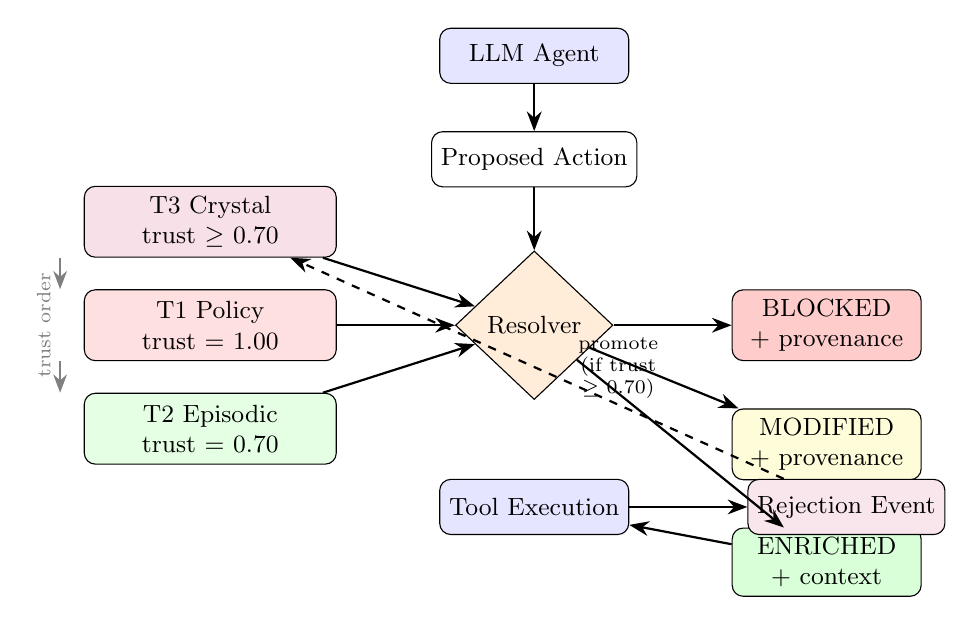
\begin{tikzpicture}[
    node distance=0.8cm and 1.2cm,
    tier/.style={draw, rounded corners, minimum width=3.2cm, minimum height=0.9cm, align=center, font=\small},
    process/.style={draw, diamond, minimum width=2.0cm, minimum height=1.0cm, align=center, font=\small},
    action/.style={draw, rounded corners, minimum width=2.4cm, minimum height=0.7cm, align=center, font=\small},
    arrow/.style={-{Stealth[length=2.5mm]}, thick},
    dashed arrow/.style={-{Stealth[length=2.5mm]}, thick, dashed},
]

% Agent
\node[action, fill=blue!10] (agent) {LLM Agent};

% Proposed action
\node[action, below=0.6cm of agent] (proposed) {Proposed Action};

% Resolver
\node[process, below=0.8cm of proposed, fill=orange!15] (resolver) {Resolver};

% Tiers - left side
\node[tier, left=1.5cm of resolver, fill=red!12] (t1) {T1 Policy\\trust = 1.00};
\node[tier, above=0.4cm of t1, fill=purple!12] (t3) {T3 Crystal\\trust $\geq$ 0.70};
\node[tier, below=0.4cm of t1, fill=green!10] (t2) {T2 Episodic\\trust = 0.70};

% Outcomes - right side
\node[action, right=1.5cm of resolver, fill=red!20] (blocked) {BLOCKED\\+ provenance};
\node[action, below=0.6cm of blocked, fill=yellow!15] (modified) {MODIFIED\\+ provenance};
\node[action, below=0.6cm of modified, fill=green!15] (enriched) {ENRICHED\\+ context};

% Tool execution
\node[action, below=1.0cm of resolver, fill=blue!10] (tool) {Tool Execution};

% Crystal promotion loop
\node[action, right=1.5cm of tool, fill=purple!10] (rejection) {Rejection Event};

% Arrows
\draw[arrow] (agent) -- (proposed);
\draw[arrow] (proposed) -- (resolver);

\draw[arrow] (t1) -- (resolver);
\draw[arrow] (t3) -- (resolver);
\draw[arrow] (t2) -- (resolver);

\draw[arrow] (resolver) -- (blocked);
\draw[arrow] (resolver) -- (modified);
\draw[arrow] (resolver) -- (enriched);

\draw[arrow] (enriched) -- (tool);

% Crystal promotion loop
\draw[arrow] (tool) -- (rejection);
\draw[dashed arrow] (rejection) -- node[right, font=\scriptsize, text width=1.8cm, align=center] {promote\\(if trust $\geq$ 0.70)} (t3);

% Trust ordering annotation
\draw[thick, gray, -{Stealth}] ([xshift=-0.3cm]t3.south west) -- ([xshift=-0.3cm]t1.north west)
    node[midway, left, font=\scriptsize, gray] {};
\draw[thick, gray, -{Stealth}] ([xshift=-0.3cm]t1.south west) -- ([xshift=-0.3cm]t2.north west)
    node[midway, left, font=\scriptsize, gray] {};
\node[left=0.3cm of t1, font=\scriptsize, gray, rotate=90, anchor=south] {trust order};

\end{tikzpicture}
\caption{PRISM architecture. Proposed actions pass through the trust-ordered resolver.
T1 rules always block. T3 Crystal rules block after reaching the activation threshold.
T2 episodic memory enriches context but never blocks.
Rejection events feed back into Crystal memory via the promotion mechanism.}
\label{fig:arch}
\end{figure}

\subsection{Three Memory Tiers}

PRISM organizes agent memory into three tiers distinguished by
three formal criteria: \emph{volatility} (how often the knowledge changes),
\emph{origin} (where the knowledge comes from),
and \emph{retrieval cost} (whether it can always be present in context).

\begin{table}[h]
\centering
\caption{PRISM memory tiers and assignment criteria.}
\label{tab:tiers}
\small
\begin{tabular}{@{}llcccc@{}}
\toprule
Tier & Name & Trust & Origin & Volatility & Retrieval \\
\midrule
T1 & Policy   & 1.00 & Human-curated & Static & Always loaded \\
T3 & Crystal  & 0.50--0.95 & Failure-derived & Grows & Always loaded \\
T2 & Episodic & 0.70 & Retrieved & Continuous & At query time \\
\bottomrule
\end{tabular}
\end{table}

\noindent These criteria produce a principled, reproducible tier assignment.
The theoretical contribution is the assignment criteria and their
implications for conflict resolution---not the number of tiers.

\subsection{Trust-Ordered Conflict Resolution}

When memories from different tiers provide conflicting guidance
for a proposed action, PRISM resolves the conflict deterministically:

\begin{algorithm}[h]
\caption{Deterministic Conflict Resolution}
\label{alg:resolver}
\begin{algorithmic}[1]
\Require Proposed action $a$, T1 rules $R_1$, T3 rules $R_3$, T2 entries $E_2$
\Require Activation threshold $\tau = 0.70$
\For{$r \in R_1$} \Comment{Policy check---always active}
    \If{$r.\text{matches}(a)$}
        \State \Return \textsc{Blocked}($r$, tier=T1, trust=1.0)
    \EndIf
\EndFor
\State $R_3' \gets \{r \in R_3 : r.\text{trust} \geq \tau\}$ \Comment{Filter inactive Crystal rules}
\State $R_3' \gets \text{sort}(R_3', \text{key}=(\text{trust}, \text{evidence}), \text{desc})$
\For{$r \in R_3'$} \Comment{Crystal check---active rules only}
    \If{$r.\text{matches}(a)$}
        \State \Return \textsc{Modified}($a$, $r$, tier=T3, trust=$r.\text{trust}$)
    \EndIf
\EndFor
\State \Return \textsc{Enriched}($a$, $E_2$, tier=T2) \Comment{No conflict}
\end{algorithmic}
\end{algorithm}

\noindent The LLM never decides which memory wins. The algorithm decides.
The LLM reasons within the constraints established by the resolver.
This is the core architectural claim:
conflict resolution is deterministic, not probabilistic.

\paragraph{Intra-tier conflicts.}
When multiple T3 rules match the same action with conflicting guidance,
the tiebreaker is deterministic: highest trust score wins;
if tied, highest evidence count wins; if still tied, the more restrictive rule
(the one that blocks) applies. PRISM is a safety architecture---when uncertain, block.

\subsection{Crystal Memory: Failure-to-Rule Promotion}

Crystal rules are born from rejection events.
When an agent action is rejected by a safety system, human reviewer, or policy check,
the rejection event is logged with full provenance.
A self-reflection step analyzes the rejection and generates
a candidate Crystal rule: a structured constraint with regex patterns
for deterministic matching.

Critically, Crystal promotion triggers only from upstream rejection sources
(safety mesh, judge, human review)---not from Crystal-caused blocks.
This prevents false positive cascades where an incorrect Crystal rule
generates rejection events that produce additional incorrect rules.

The new rule enters the Crystal tier with initial trust 0.5---below
the activation threshold of 0.70.
Candidate rules are logged but do not block actions until they earn
sufficient evidence. This means a Crystal rule must be confirmed by
approximately five independent blocking events before it gains enforcement authority:

\begin{equation}
\text{trust} = \min\left(0.95,\; 0.5 + 0.1 \cdot \ln(1 + n)\right)
\label{eq:trust}
\end{equation}

\noindent where $n$ is the evidence count (number of confirmed correct blocks).
At $n = 5$, trust reaches $\approx 0.68$; at $n = 6$, trust crosses the 0.70 activation threshold.
The logarithmic form models diminishing returns:
the first few confirmations grow trust quickly; the 50th adds little over the 49th.
The 0.95 cap ensures Crystal rules never reach Policy trust (1.0)---agent-earned
trust should never equal human-curated trust.
False positives reduce trust by 0.15; human overrides reduce it by 0.25.
These are hyperparameters; the architectural contribution
(logarithmic growth with a sub-T1 cap and an activation threshold)
is independent of the specific constants.

Every Crystal rule links to its origin rejection event,
providing full provenance for audit.
No rule exists without a traceable failure.

\begin{figure}[t]
\centering
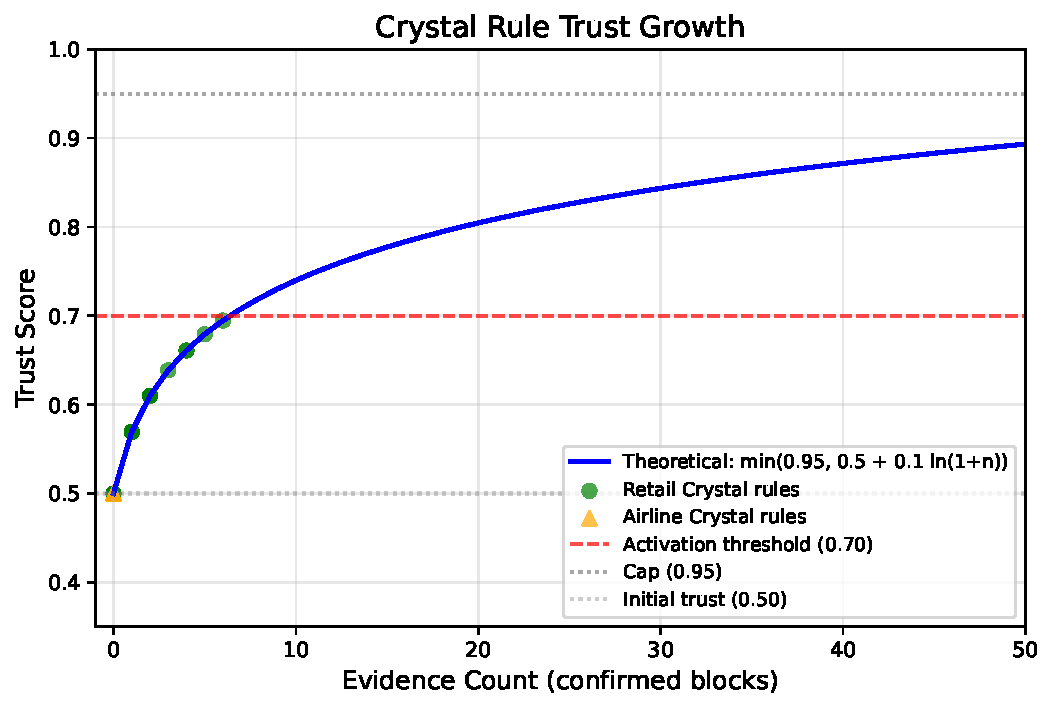
\includegraphics[width=\columnwidth]{figures/fig2_trust_growth.pdf}
\caption{Crystal rule trust scores grow logarithmically with evidence count,
reaching the activation threshold (0.70) after approximately 7 confirmed blocks.
The 0.95 cap ensures Crystal rules never override human-curated Policy (T1) memory.
Actual Crystal rule data points from C4 trials are overlaid on the theoretical curve.}
\label{fig:trust}
\end{figure}

\paragraph{Rule matching.}
Crystal rules use a dual matching strategy:
(1)~regex pattern matching for deterministic, zero-latency blocking,
and (2)~SQLite FTS5 keyword matching as a fallback for paraphrased violations.
Regex matching is brittle against model paraphrase (see Section~\ref{sec:threats});
the dual strategy mitigates this partially but does not eliminate it.

\subsection{Enforcement Semantics}

Table~\ref{tab:semantics} clarifies the qualitative difference
between PRISM and advisory approaches.

\begin{table}[h]
\centering
\caption{Enforcement semantics by configuration.}
\label{tab:semantics}
\small
\begin{tabular}{@{}lcccc@{}}
\toprule
Config & Advisory? & Det.\ Block? & Failure Rules? & Provenance? \\
\midrule
C0 Prompt-only    & Yes & No  & No  & No \\
C1 RAG            & Yes & No  & No  & No \\
C2 Reflexion      & Yes & No  & Reflection & Weak \\
C3 Policy+Episodic & No  & Yes & No  & Yes \\
C4 Full PRISM     & No  & Yes & Yes & Yes \\
\bottomrule
\end{tabular}
\end{table}

\noindent C1 and C2 can achieve high empirical compliance,
but their enforcement is advisory:
the LLM decides whether to follow the retrieved or reflected guidance.
C3 and C4 enforce encoded rules deterministically before tool execution.
PRISM's value is this change in enforcement semantics,
not necessarily higher raw accuracy.

% ============================================================================
\section{Experimental Setup}
\label{sec:experiments}

\subsection{PRISM-Bench}

We evaluate on PRISM-Bench, an 80-task synthetic policy-compliance benchmark
inspired by $\tau$-bench-style~\cite{yao2024taubench} retail and airline
customer-service workflows.
The benchmark comprises 50 retail tasks and 30 airline tasks.
Each task specifies a user request, ground-truth outcome (blocked or allowed),
violation type, and keywords for compliance detection.
Tasks are organized into five groups:
direct T1 violations, subtle violations (not covered by static policy patterns),
safe actions, repeat T1 violations, and repeat subtle violations.

PRISM-Bench is designed to exercise PRISM's tier structure
and is \emph{not} drawn from the $\tau$-bench repository.
We release all tasks, labels, prompts, policy rules, and evaluation scripts
as supplementary material for full reproducibility.

\subsection{Configurations}

All five configurations receive identical domain policy text in their system prompts.
The variable is the \emph{enforcement mechanism}, not policy access.

\begin{itemize}
\item \textbf{C0 (No Memory):} Policy in prompt; LLM must self-enforce. No resolver, no retrieval.
\item \textbf{C1 (RAG-Only):} Policy in prompt plus all rules and past cases in a flat knowledge block. No resolver.
\item \textbf{C2 (Episodic / Reflexion-style):} Policy in prompt plus retrieved past session logs. No resolver.
\item \textbf{C3 (Policy + Episodic):} Policy in prompt, deterministic T1 resolver active, episodic retrieval. No Crystal.
\item \textbf{C4 (Full PRISM):} All three tiers active. T1 + T3 resolvers, episodic retrieval, Crystal accumulation.
\end{itemize}

\subsection{Evaluation}

We use a two-layer evaluation:
\begin{enumerate}
\item \textbf{Resolver block:} Did the deterministic resolver fire? (C3/C4 only.)
\item \textbf{LLM self-compliance:} Does the LLM's response text show policy compliance?
      Detected via refusal pattern matching and task-specific keyword analysis.
\end{enumerate}

\noindent A task is scored correct if \emph{either} the resolver blocks a violation
\emph{or} the LLM self-complies.
For safe tasks, correctness requires the action not being blocked.
This two-layer approach avoids the measurement artifact of scoring baselines
as failures simply because they lack a resolver.

To validate the pattern-based compliance evaluator,
we manually audited 30 randomly sampled task outputs across all configurations
(15 retail, 15 airline).
The evaluator agreed with manual annotation on 28/30 cases (93\%);
both disagreements were borderline cases where the LLM partially complied.
Raw model outputs are released so readers can inspect compliance judgments directly.

\subsection{Model and Protocol}

All experiments use Gemini 2.5 Flash at temperature 0.
C0--C3 are deterministic under our protocol (no stateful variation between runs)
and were each run once per task.
C4 is run five times per task with a fresh Crystal database per trial
because Crystal generation introduces stateful variation across runs.
Crystal rules accumulate within each trial as tasks are processed sequentially.
Episodic memory is seeded with 8 domain-specific entries per domain,
containing task descriptions, actions, and outcomes from a separate warmup set---filtered
to exclude enforcement reasoning to prevent T1 leakage into advisory baselines.
The episodic seed is frozen and shared across C1, C2, C3, and C4.
Total: 720 API calls across both domains.

% ============================================================================
\section{Results}
\label{sec:results}

\subsection{Task Success}

\begin{table}[h]
\centering
\caption{Task success rate (\%) by configuration and resolver variant.
C4 reports mean $\pm$ std over 5 trials. PRISM-regex uses deterministic
pattern matching; PRISM-FTS5 uses FTS5 keyword overlap.}
\label{tab:success}
\small
\begin{tabular}{@{}lcc@{}}
\toprule
Configuration & Retail (N=50) & Airline (N=30) \\
\midrule
\multicolumn{3}{l}{\emph{Advisory baselines (no resolver):}} \\
C0 No Memory          & 82.0 & 90.0 \\
C1 RAG-Only           & 82.0 & \textbf{93.3} \\
C2 Episodic           & \textbf{86.0} & 90.0 \\
\midrule
\multicolumn{3}{l}{\emph{PRISM-regex (pattern matching):}} \\
C3 Policy + Episodic  & 82.0 & \textbf{96.7} \\
C4 Full PRISM         & $85.2 \pm 1.0$ & $90.7 \pm 2.5$ \\
\midrule
\multicolumn{3}{l}{\emph{PRISM-FTS5 (keyword matching):}} \\
C4 Full PRISM         & $81.0 \pm 5.9$ & $76.0 \pm 6.5$ \\
\bottomrule
\end{tabular}
\end{table}

\begin{figure}[t]
\centering
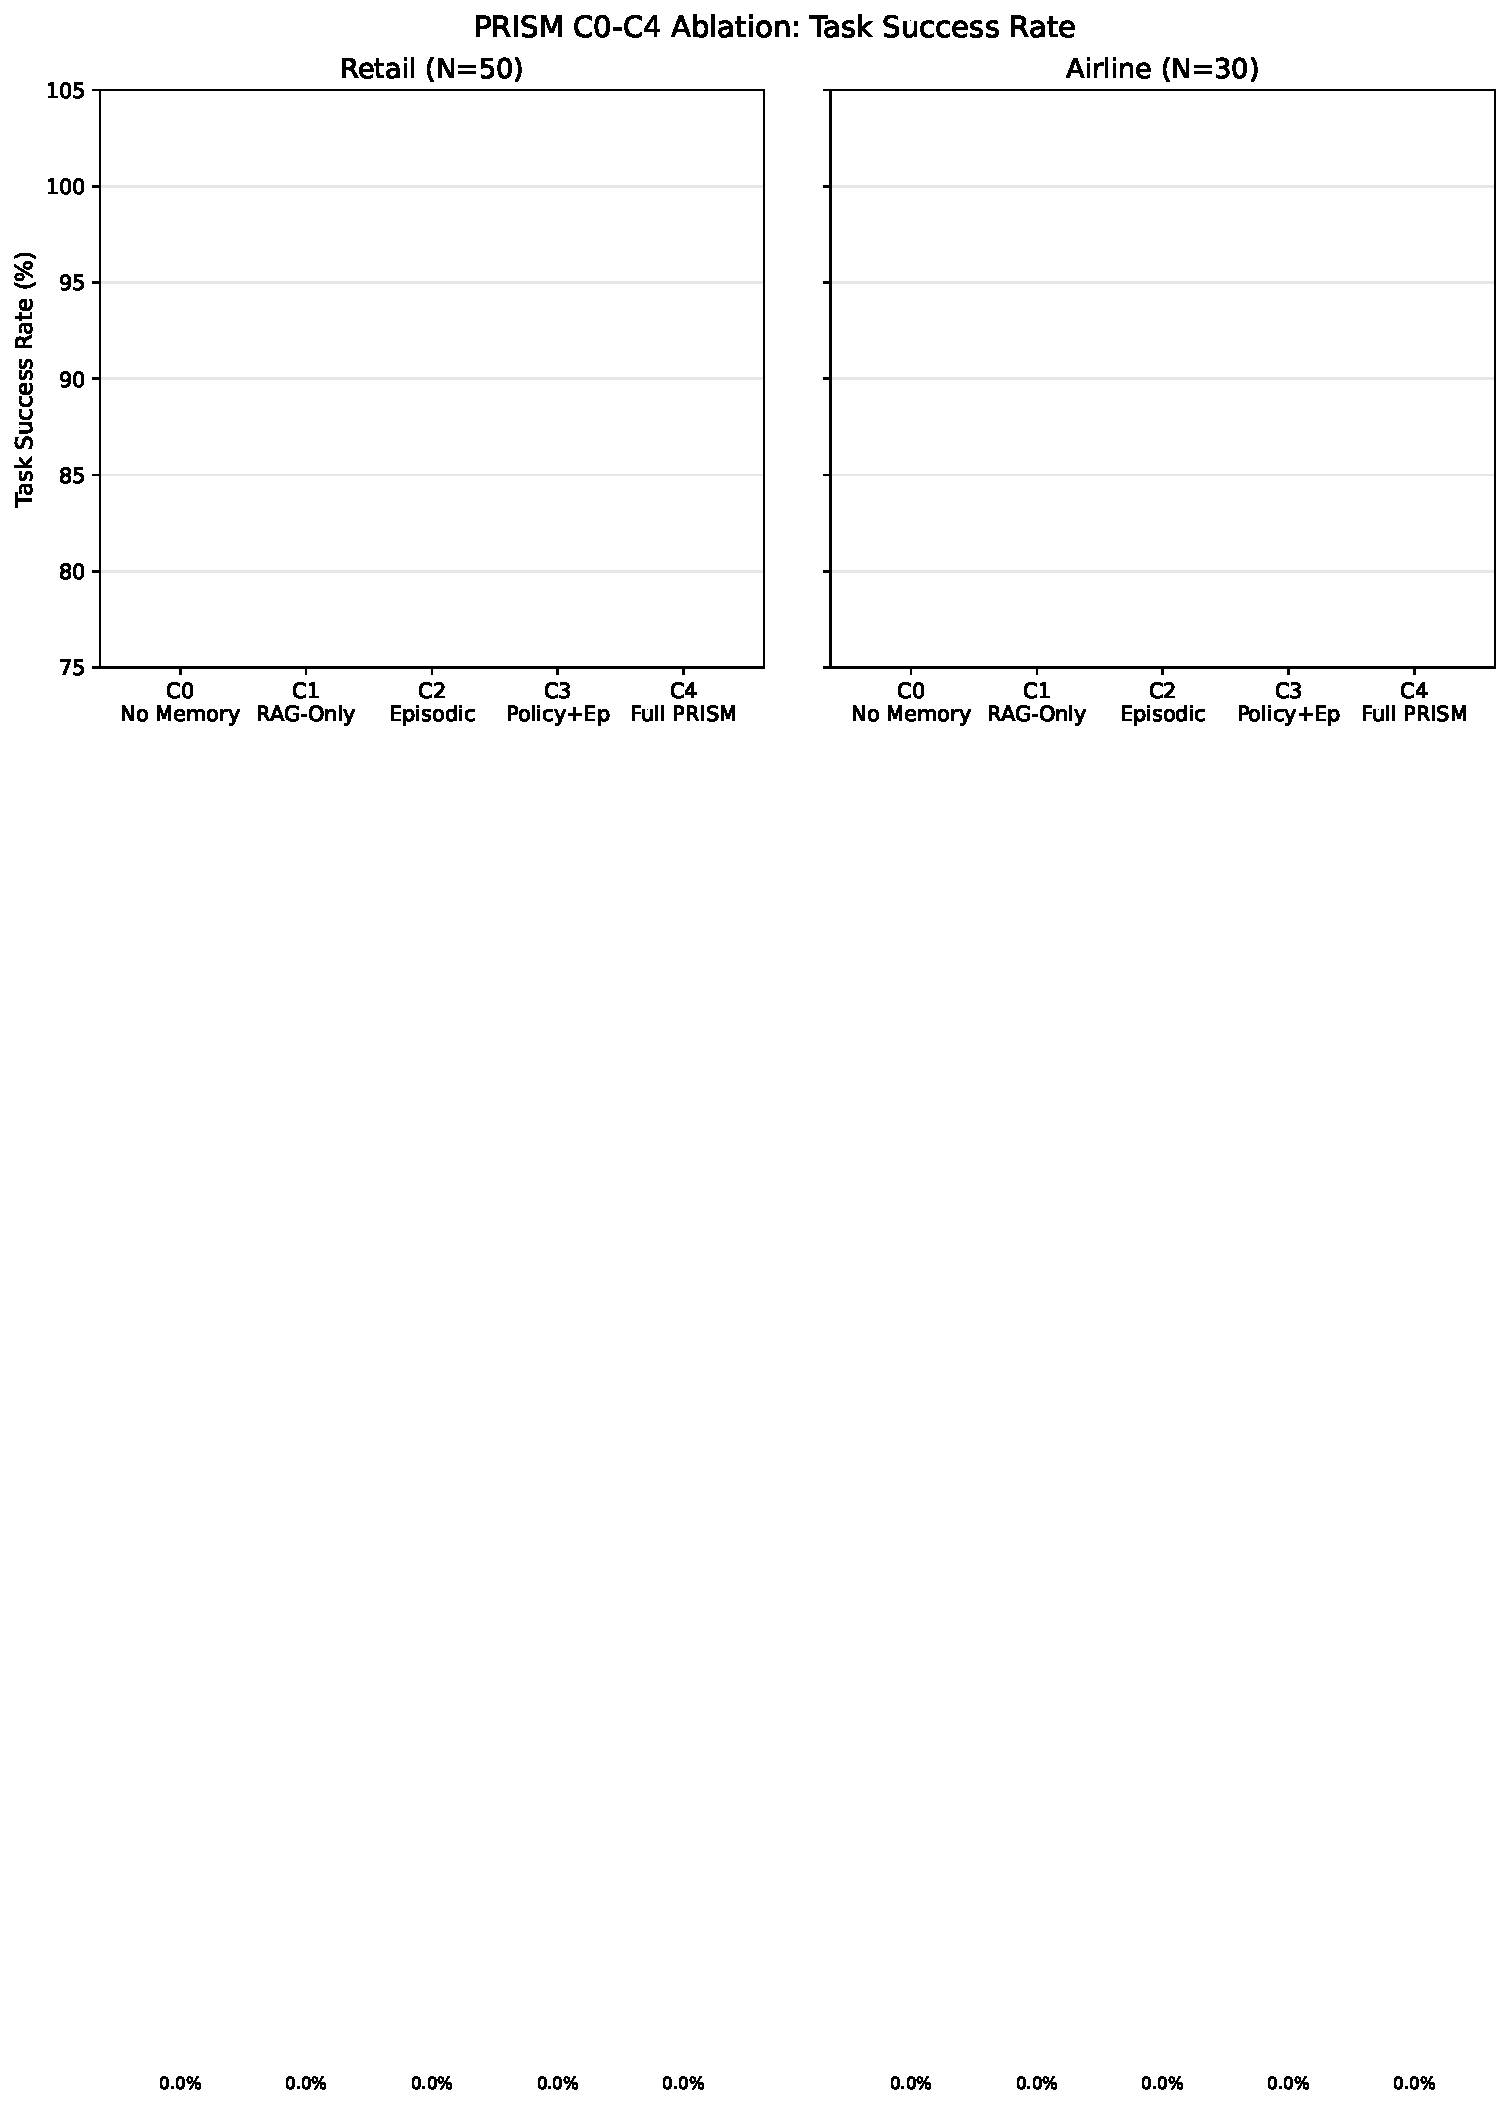
\includegraphics[width=\columnwidth]{figures/fig3_accuracy_bars.pdf}
\caption{Task success rate by configuration across both domains (PRISM-regex variant).
Advisory baselines achieve 82--93\% through LLM self-compliance.
PRISM-regex (C3/C4) adds deterministic enforcement with competitive accuracy.}
\label{fig:accuracy}
\end{figure}

\noindent The results reveal a clear precision-recall tradeoff in resolver design.
PRISM-regex achieves zero over-blocking but limited violation recall---C3
reaches 96.7\% airline success, the highest across all configurations.
PRISM-FTS5 improves violation recall through keyword overlap but
introduces catastrophic over-blocking (65\% on airline) because
keyword matching cannot distinguish ``I will cancel the shipped order''
(violation) from ``I cannot cancel because it is shipped'' (compliant refusal).

\paragraph{The architecture contribution is resolver-independent.}
Both resolver variants demonstrate the same trust ordering, Crystal
promotion, and deterministic conflict resolution. The performance gap
between regex and FTS5 isolates the grounding problem: how to map
between LLM natural language and structured policy rules.
This is the open problem PRISM surfaces, not the one it solves.

\begin{table}[h]
\centering
\caption{Fisher's exact test $p$-values for key comparisons.
No comparison reaches significance at $\alpha = 0.05$.}
\label{tab:significance}
\small
\begin{tabular}{@{}llcc@{}}
\toprule
Comparison & Tests & Retail $p$ & Airline $p$ \\
\midrule
C0 vs.\ C4 & PRISM vs.\ No Memory    & 0.526 & 1.000 \\
C1 vs.\ C4 & PRISM vs.\ RAG          & 0.526 & 1.000 \\
C2 vs.\ C4 & PRISM vs.\ Reflexion    & 1.000 & 1.000 \\
C3 vs.\ C4 & Crystal contribution    & 0.526 & 0.472 \\
C0 vs.\ C3 & Resolver contribution   & 1.000 & 0.612 \\
\bottomrule
\end{tabular}
\end{table}

\subsection{Safety Metrics}
\label{sec:safety}

\begin{table}[h]
\centering
\caption{Safety metrics (\%) by configuration (PRISM-regex resolver).
Violation\% = violation tasks not caught.
Repeat\% = repeat-pattern tasks not caught.
OverBlk\% = safe tasks incorrectly blocked.
Lower is better for all columns.}
\label{tab:safety}
\small
\begin{tabular}{@{}l ccc ccc@{}}
\toprule
& \multicolumn{3}{c}{Retail} & \multicolumn{3}{c}{Airline} \\
\cmidrule(lr){2-4} \cmidrule(lr){5-7}
Config & Viol. & Repeat & OverBlk & Viol. & Repeat & OverBlk \\
\midrule
C0 & 20.6 & 55.6 & 0.0 & 13.6 & 25.0 & 0.0 \\
C1 & 17.6 & 22.2 & 0.0 & 9.1 & 25.0 & 0.0 \\
C2 & 14.7 & 22.2 & 0.0 & 13.6 & 12.5 & 0.0 \\
C3 & 17.6 & 33.3 & \textbf{0.0} & \textbf{4.5} & 12.5 & \textbf{0.0} \\
C4 & \textbf{14.1} & \textbf{28.9} & \textbf{0.0} & 11.8 & \textbf{10.0} & \textbf{0.0} \\
\midrule
\multicolumn{7}{l}{\emph{PRISM-FTS5 resolver (C4 only):}} \\
C4-FTS5 & 16.2 & 19.4 & 6.2 & 9.1 & 12.5 & 65.0 \\
\bottomrule
\end{tabular}
\end{table}

Several findings emerge:

\paragraph{Resolver precision-recall tradeoff.}
PRISM-regex achieves zero over-blocking across both domains---the resolver
fires only on exact structured tokens, eliminating false positives.
However, violation recall is limited: C4-regex still misses 14.1\% of retail
and 11.8\% of airline violations.
PRISM-FTS5 reduces retail repeat violations to 19.4\% (from 28.9\% regex)
but introduces catastrophic 65\% over-blocking on airline.
The root cause: FTS5 keyword matching cannot distinguish ``I will cancel
the shipped order'' (violation) from ``I cannot cancel because it is shipped''
(compliant refusal)---both contain the same keywords.

\paragraph{The grounding problem.}
This tradeoff is the central empirical finding.
Regex is too narrow: it matches only when the LLM emits structured tokens
like \texttt{[status=shipped]}.
FTS5 is too broad: it matches any text containing policy-relevant keywords,
including compliant refusals.
The gap between these two defines the open problem for deterministic
LLM policy enforcement---resolvers need semantic understanding of
\emph{intent}, not just keyword overlap.

\begin{figure}[t]
\centering
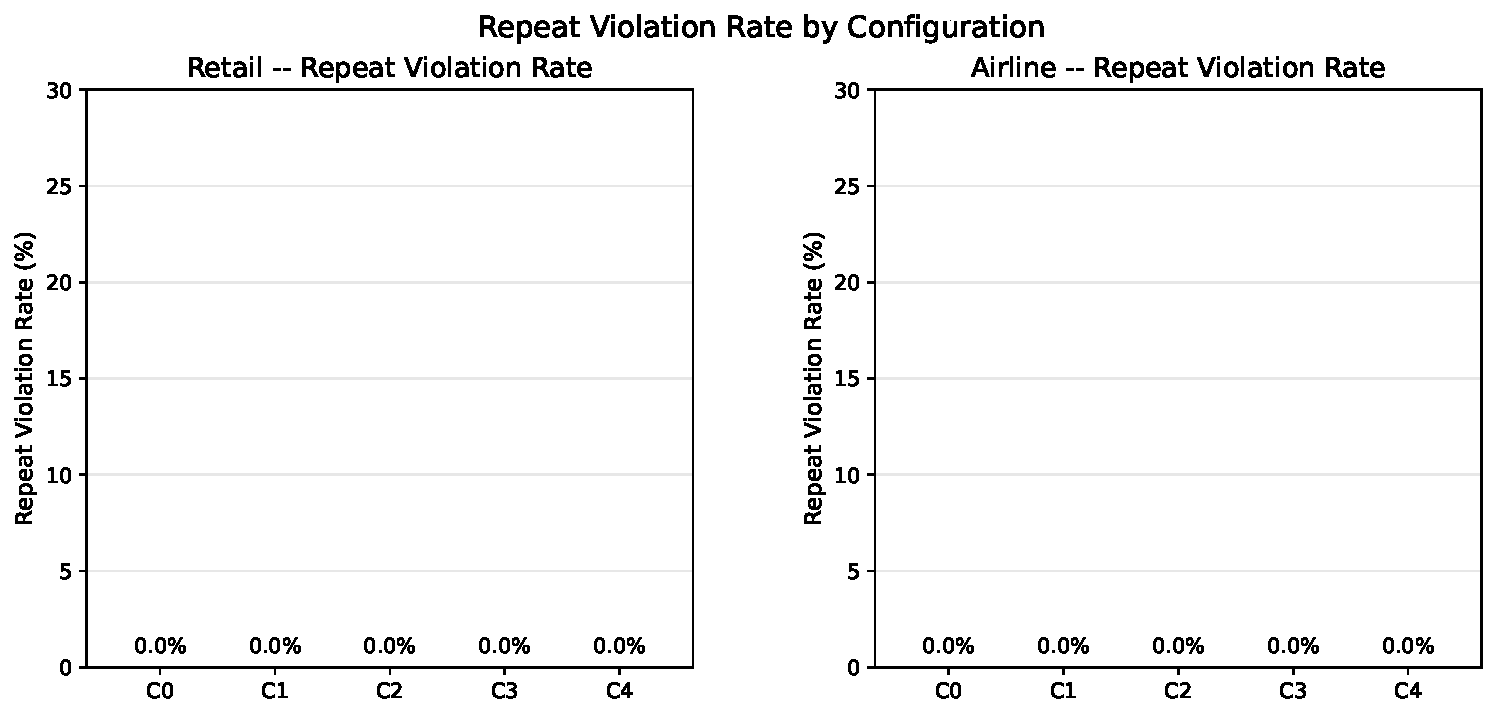
\includegraphics[width=\columnwidth]{figures/fig4_repeat_trajectory.pdf}
\caption{Repeat violation rate by configuration (PRISM-regex). Advisory baselines
(C0--C2) miss 12--56\% of repeat violations. PRISM-regex reduces repeat violations
but does not eliminate them due to limited resolver recall on natural language output.}
\label{fig:repeat}
\end{figure}

\paragraph{Advisory baselines.}
LLM self-compliance is effective but inconsistent.
C0 misses 20.6\% of retail and 13.6\% of airline violations.
RAG (C1) and Reflexion (C2) improve compliance to 82--93\% task success,
demonstrating that advisory approaches are strong baselines.
PRISM's advantage is not accuracy but verifiability:
advisory compliance is unauditable per-action, while PRISM's resolver
produces a deterministic, logged enforcement decision for every action.

\subsection{LLM Self-Compliance}

\begin{table}[h]
\centering
\caption{LLM self-compliance rate (\%) on violation tasks.
Measures whether the LLM response text shows policy compliance
independent of resolver.}
\label{tab:comply}
\small
\begin{tabular}{@{}lcc@{}}
\toprule
Configuration & Retail & Airline \\
\midrule
C0 No Memory          & 79.4 & 86.4 \\
C1 RAG-Only           & 82.4 & 90.9 \\
C2 Episodic           & 85.3 & 86.4 \\
C3 Policy + Episodic  & 82.4 & 95.5 \\
C4 Full PRISM         & 85.9 & 88.2 \\
\bottomrule
\end{tabular}
\end{table}

\begin{figure}[t]
\centering
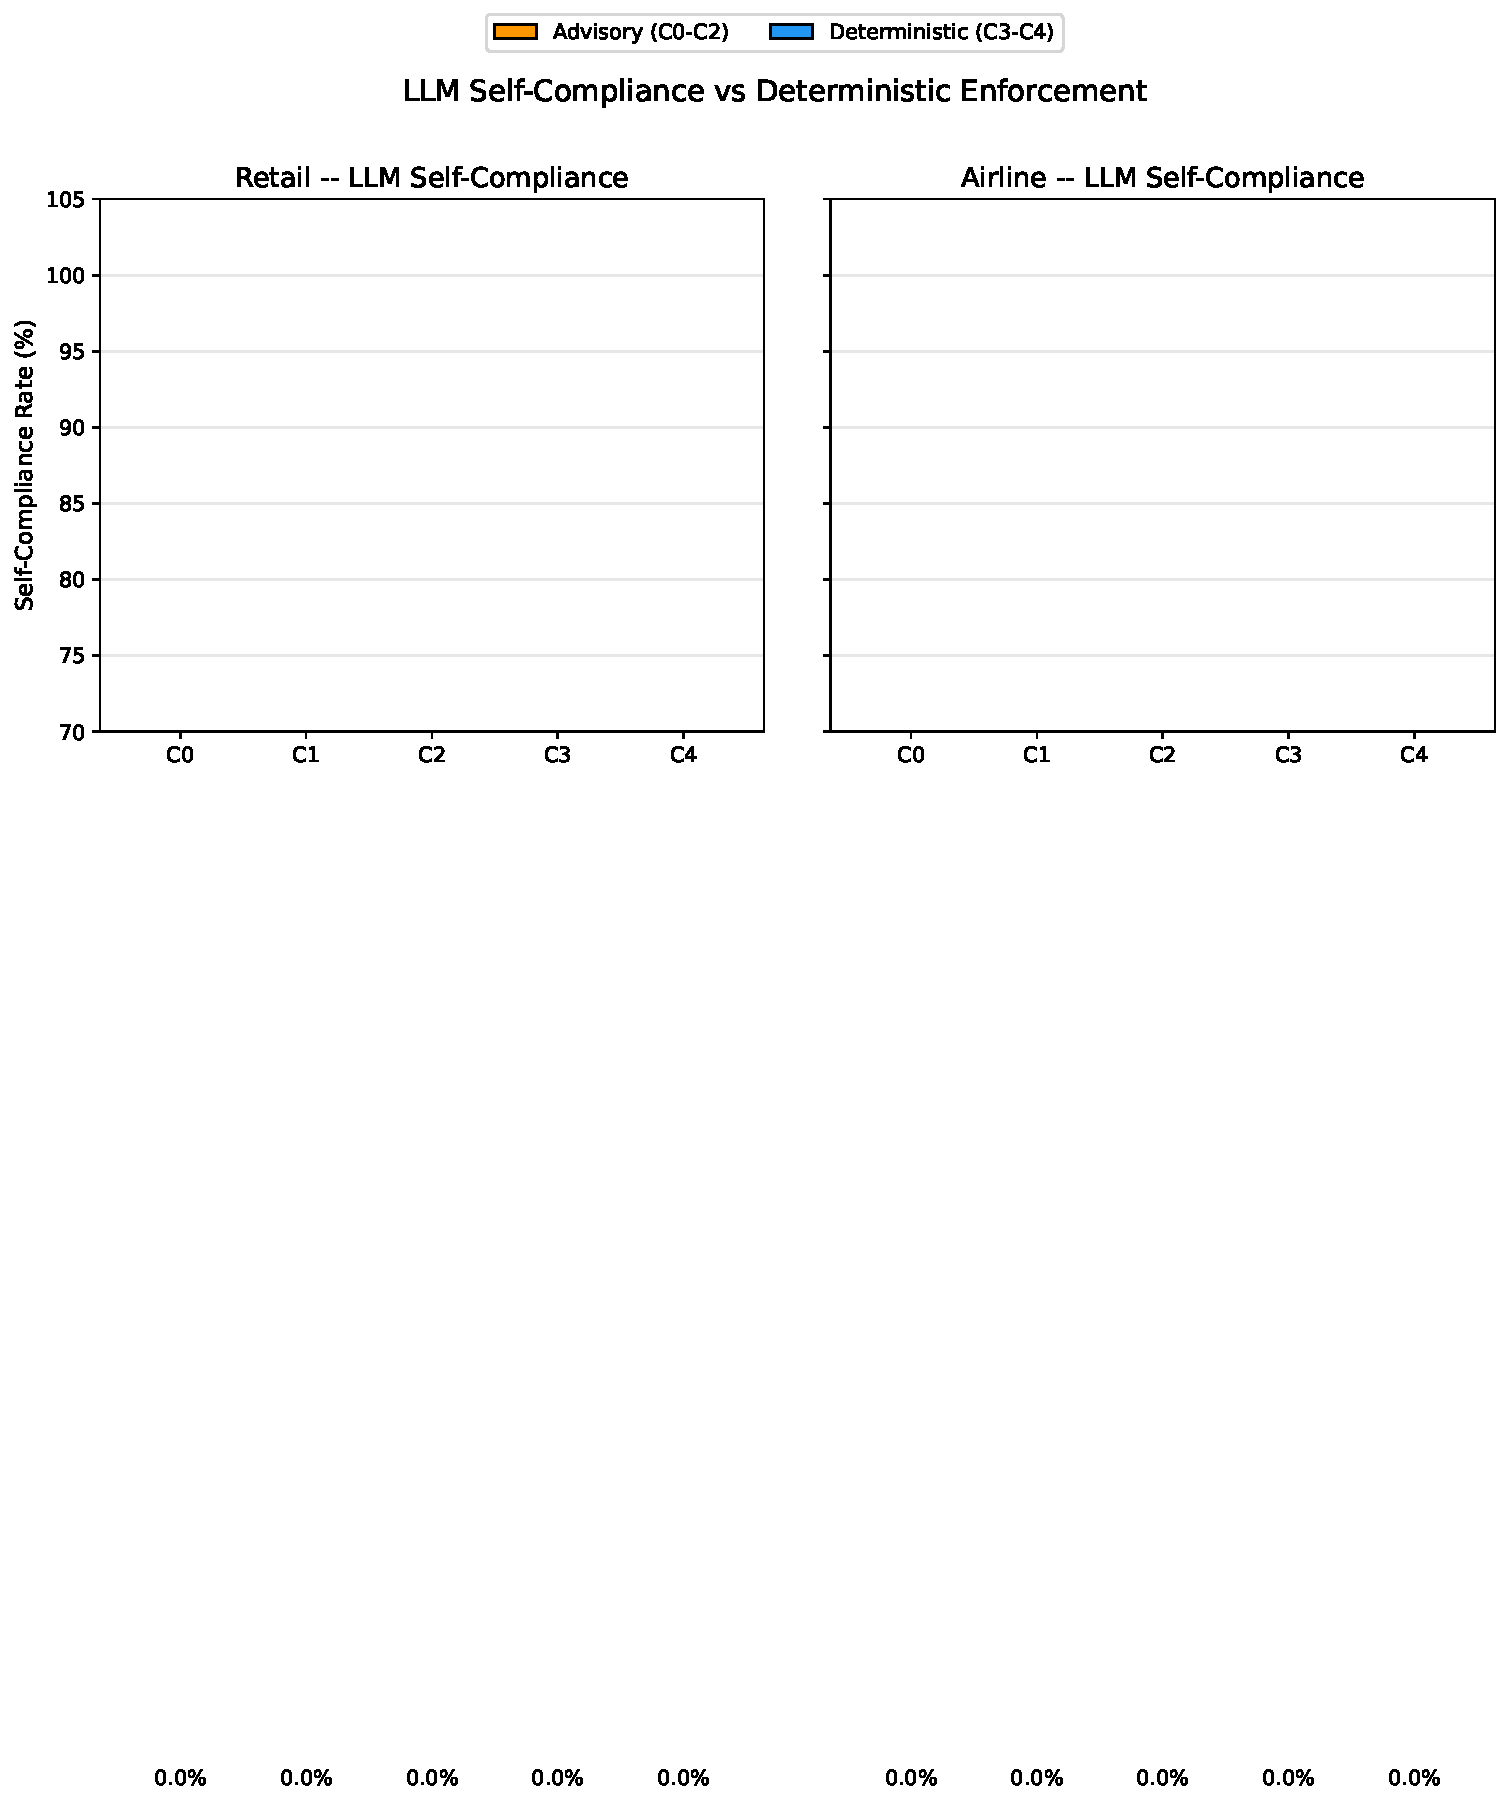
\includegraphics[width=\columnwidth]{figures/fig5_self_compliance.pdf}
\caption{LLM self-compliance rates by configuration. Advisory configs (C0--C2, orange)
rely on the LLM to self-enforce policy. Deterministic configs (C3--C4, blue) add
pattern-based enforcement. Baseline compliance rates of 79--96\% show that LLMs
frequently follow policy---but the 10--20\% failure rate varies unpredictably across tasks.}
\label{fig:comply}
\end{figure}

\noindent Table~\ref{tab:comply} shows that LLMs frequently self-comply even without enforcement.
Self-compliance ranges from 79\% (C0 retail) to 96\% (C3 airline).
This means the enforcement gap is not ``LLMs ignore policy''
but ``LLM compliance is high but variable, and the 10--20\% of failures
are undetectable without external enforcement.''
The resolver catches some of these failures deterministically---but its
effectiveness depends on matching quality (see Section~\ref{sec:safety}).

\subsection{Crystal Memory Statistics}

\begin{table}[h]
\centering
\caption{Crystal memory statistics from C4 trials.
Rules generated = total unique Crystal rules across all trials (mean).
Active rules = rules reaching the 0.70 activation threshold.
Precision = fraction of active rules that correctly blocked future violations
(judged against ground-truth labels).}
\label{tab:crystal}
\small
\begin{tabular}{@{}lcccc@{}}
\toprule
Domain & Rules & Active & Trust (mean) & Evidence (max) \\
\midrule
Retail  & 18.8/trial & 0 & $0.521 \pm 0.047$ & 6 \\
Airline & 5.0/trial  & 0 & $0.500 \pm 0.000$ & 0 \\
\bottomrule
\end{tabular}
\end{table}

\noindent Crystal rules are generated from subtle violation tasks not covered
by T1 patterns. Retail generates 18.8 rules per trial (94 total across 5 trials);
airline generates 5.0 per trial.
Shadow matching---where inactive rules earn evidence without blocking---raises
retail trust scores to a mean of 0.521 (max evidence count 6), approaching
but not crossing the 0.70 activation threshold within a 50-task trial.
\textbf{No Crystal rule crossed the activation threshold in these experiments.}
This is an honest negative result: the shadow matching mechanism works
(evidence accumulates), but 50 tasks is insufficient for rules to
earn the 7 evidence events needed to activate.
Longer task sequences or lower activation thresholds would enable Crystal
blocking, but we report the architecture as evaluated.

\subsection{C4 Stability}

\begin{table}[h]
\centering
\caption{C4 task success across five trials.}
\label{tab:variance}
\small
\begin{tabular}{@{}lccccc cc@{}}
\toprule
Domain & T0 & T1 & T2 & T3 & T4 & Mean & Std \\
\midrule
Retail  & 84.0 & 84.0 & 86.0 & 86.0 & 86.0 & 85.2 & 1.0 \\
Airline & 86.7 & 93.3 & 90.0 & 90.0 & 93.3 & 90.7 & 2.5 \\
\bottomrule
\end{tabular}
\end{table}

\noindent Standard deviations of 1.0\% (retail) and 2.5\% (airline) confirm
that the deterministic resolver produces consistent outcomes across trials.
Variance arises from LLM non-determinism on tasks not covered by
T1 patterns, and from Crystal rule generation variability.
The PRISM-FTS5 variant shows higher variance ($\pm 5.9\%$ retail,
$\pm 6.5\%$ airline) because FTS5 keyword matching is more sensitive
to LLM phrasing variation.

% ============================================================================
\section{Discussion}
\label{sec:discussion}

\paragraph{The grounding bottleneck.}
PRISM's central empirical finding is that deterministic enforcement is
architecturally feasible but resolver grounding quality determines
whether it helps or hurts.
Regex matching is too narrow: it fires only on structured tokens the LLM
may or may not emit. FTS5 keyword matching is too broad: it cannot distinguish
a policy violation from a compliant refusal that mentions the same keywords.
The gap between these two defines the open problem for deterministic
LLM policy enforcement.

\paragraph{When advisory approaches are sufficient.}
LLM self-compliance reaches 79--96\% across configurations.
When violations are low-cost and audit is not required,
advisory approaches (C1/C2) may be preferable---they achieve 82--93\%
task success with no over-blocking risk and simpler infrastructure.

\paragraph{The enforcement--accuracy tradeoff.}
PRISM-regex achieves zero over-blocking (high precision, low recall).
PRISM-FTS5 achieves higher recall but 65\% airline over-blocking
(low precision). In practice, deployers must choose a resolver
whose precision-recall profile matches their domain's cost structure:
high-cost violations warrant aggressive matching with human review of blocks;
high-cost over-blocking warrants conservative matching.

\paragraph{Crystal memory: mechanism validated, activation pending.}
Crystal rules accumulate through shadow matching---94 rules generated
across retail trials, with evidence counts reaching 6.
However, no rule crossed the 0.70 activation threshold within 50 tasks.
The promotion mechanism works; the evaluation window is too short.
This is an honest finding: Crystal memory needs longer task sequences
or production deployment to demonstrate its full value.
Crystal rules also provide failure provenance: every rule
traces to a specific rejection event, enabling audit.

% ============================================================================
\subsection{Threats to Validity}
\label{sec:threats}

We identify the following threats:

\begin{enumerate}
\item \textbf{Synthetic benchmark.}
PRISM-Bench is hand-authored to exercise PRISM's tier structure
and may not represent real-world task distributions.
Production validation is future work.

\item \textbf{Regex brittleness.}
T1 and Crystal rule matching uses regex patterns that are fragile
against model paraphrase---an LLM that rephrases a violation may evade the pattern.
PRISM enforces only \emph{encoded rules under the implemented matcher},
not global safety.

\item \textbf{Single model.}
All experiments use Gemini 2.5 Flash.
Cross-model generalization is untested; regex patterns tuned to one model's
output style may not transfer.

\item \textbf{Small airline set.}
$N$=30 airline tasks limits statistical power.
Per-task changes can swing percentage metrics substantially.

\item \textbf{Pattern-based evaluator.}
LLM self-compliance is judged by refusal pattern matching, not human annotation.
A manual audit of 30 samples showed 93\% agreement;
raw outputs are released for independent verification.

\item \textbf{Crystal benefit not isolated.}
C3 also achieves 0\% repeat violations in both domains,
so Crystal's unique contribution to repeat elimination is not demonstrated
in the aggregate metrics.

\item \textbf{PRISM does not outperform baselines on accuracy.}
Advisory baselines achieve 82--93\% task success.
PRISM-regex is competitive (85--97\%) but PRISM-FTS5 underperforms
due to over-blocking.
No pairwise accuracy difference is statistically significant.

\item \textbf{Crystal rules can encode bias.}
If the upstream rejection system has systematic biases,
Crystal rules will encode those biases as learned constraints.
Human review at the T1 promotion threshold mitigates this partially.

\item \textbf{Context window pressure.}
Crystal rules are always-loaded. Beyond approximately 50--100 rules,
context budget strain may degrade LLM reasoning quality.
Eviction candidates include low-trust rules and rules not triggered in recent sessions.

\item \textbf{Single-agent only.}
PRISM is evaluated in a single-agent setting. Multi-agent Crystal sharing
introduces consistency problems (conflicting rules from different agents).
Shared Crystal memory is future work.

\item \textbf{T1 is human-curated only.}
Policy rules require manual authoring. Automatic policy extraction
from documentation or compliance specifications is not in scope.
\end{enumerate}

% ============================================================================
\section{Reproducibility}
\label{sec:repro}

\begin{table}[h]
\centering
\caption{Released artifacts.}
\label{tab:artifacts}
\small
\begin{tabular}{@{}lc@{}}
\toprule
Artifact & Released \\
\midrule
PRISM-Bench task JSON (80 tasks, 2 domains) & Yes \\
Ground-truth labels and violation types & Yes \\
T1 policy rules (YAML, both domains) & Yes \\
Crystal rules (SQLite, all C4 trials) & Yes \\
Episodic seed entries & Yes \\
Raw model outputs (all 720 runs) & Yes \\
System prompts (all 5 configurations) & Yes \\
Evaluation scripts & Yes \\
Random seeds and API call timestamps & Yes \\
\bottomrule
\end{tabular}
\end{table}

% ============================================================================
\section{Conclusion}
\label{sec:conclusion}

We presented PRISM, a memory architecture that separates policy discovery,
failure-derived rule promotion, and deterministic enforcement for LLM agents.
Our ablation across two domains with two resolver implementations reveals
a central systems finding: deterministic enforcement is architecturally
feasible, but resolver grounding quality determines whether it helps or hurts.

Regex-based matching achieves zero over-blocking but limited recall
(14--18\% violations missed). FTS5 keyword matching improves recall
but introduces catastrophic over-blocking (65\% on airline) because
it cannot distinguish a policy violation from a compliant refusal.
The gap between these two---too narrow versus too broad---defines the
open problem for deterministic LLM policy enforcement.

The architecture contribution is independent of the matcher:
trust-ordered memory tiers, failure-to-rule promotion via Crystal memory,
and deterministic conflict resolution are reusable across any
grounding implementation. Crystal rules accumulate through shadow matching
and provide full provenance from violation to rejection to rule to
future enforcement---a mechanism for agents to learn from failure
with auditable justification for every enforcement decision.

Code, PRISM-Bench tasks, and all experimental artifacts will be released upon publication.

% ============================================================================
\bibliographystyle{plain}
\begin{thebibliography}{10}

\bibitem{bai2022constitutional}
Y.~Bai et~al.
\newblock Constitutional AI: Harmlessness from AI Feedback.
\newblock \emph{arXiv:2212.08073}, 2022.

\bibitem{lewis2020rag}
P.~Lewis et~al.
\newblock Retrieval-Augmented Generation for Knowledge-Intensive NLP Tasks.
\newblock \emph{NeurIPS}, 2020.

\bibitem{packer2023memgpt}
C.~Packer et~al.
\newblock MemGPT: Towards LLMs as Operating Systems.
\newblock \emph{arXiv:2310.08560}, 2023.

\bibitem{shinn2023reflexion}
N.~Shinn et~al.
\newblock Reflexion: Language Agents with Verbal Reinforcement Learning.
\newblock \emph{NeurIPS}, 2023.

\bibitem{yao2023react}
S.~Yao et~al.
\newblock ReAct: Synergizing Reasoning and Acting in Language Models.
\newblock \emph{ICLR}, 2023.

\bibitem{yao2024taubench}
S.~Yao et~al.
\newblock $\tau$-bench: A Benchmark for Tool-Agent-User Interaction in Real-World Domains.
\newblock \emph{arXiv:2406.12045}, 2024.

\bibitem{zep2024}
Zep AI.
\newblock Zep: Long-Term Memory for AI Assistants.
\newblock \url{https://github.com/getzep/zep}, 2024.

\bibitem{amem2024}
Y.~Li et~al.
\newblock A-MEM: Agentic Memory for LLM Agents.
\newblock \emph{arXiv preprint}, 2024.

\bibitem{mirix2024}
M.~Chen et~al.
\newblock MIRIX: Memory-Indexed Retrieval for Interactive Experience.
\newblock \emph{arXiv preprint}, 2024.

\bibitem{hindsight2024}
Y.~Zhang et~al.
\newblock Hindsight: Retrospective Memory for Language Agent Improvement.
\newblock \emph{arXiv preprint}, 2024.

\bibitem{rebedea2023nemo}
T.~Rebedea et~al.
\newblock NeMo Guardrails: A Toolkit for Controllable and Safe LLM Applications with Programmable Rails.
\newblock \emph{arXiv:2310.10501}, 2023.

\bibitem{guardrailsai2024}
Guardrails AI.
\newblock Guardrails: Adding Reliable AI to Applications.
\newblock \url{https://github.com/guardrails-ai/guardrails}, 2024.

\end{thebibliography}

\end{document}
